\section{Introduction}
\label{sec:intro}

Online discussions about contentious issues are increasingly shaped by coordinated influence operations. Adversaries use emotionally charged stories, manufactured doubt, and false claims of consensus to push group opinion in directions that ordinary dialogue would not produce~\citep{Tucker2018,Wardle2017,Ferrara2016}, and large language models have made such operations even cheaper~\citep{Bai2025,Salvi2025}. We call such deliberate injections of strategically framed content \emph{narrative attacks}: disruptions that work through the persuasive power of stories, emotions, and constructed credibility rather than simple falsehood. Figure~\ref{fig:motivation} illustrates the resulting threat, where a small number of attackers plant strategy-shaped messages and the ongoing reactions of neighbours carry the framing far beyond the original posts.

\begin{figure}[!t]
  \centering
  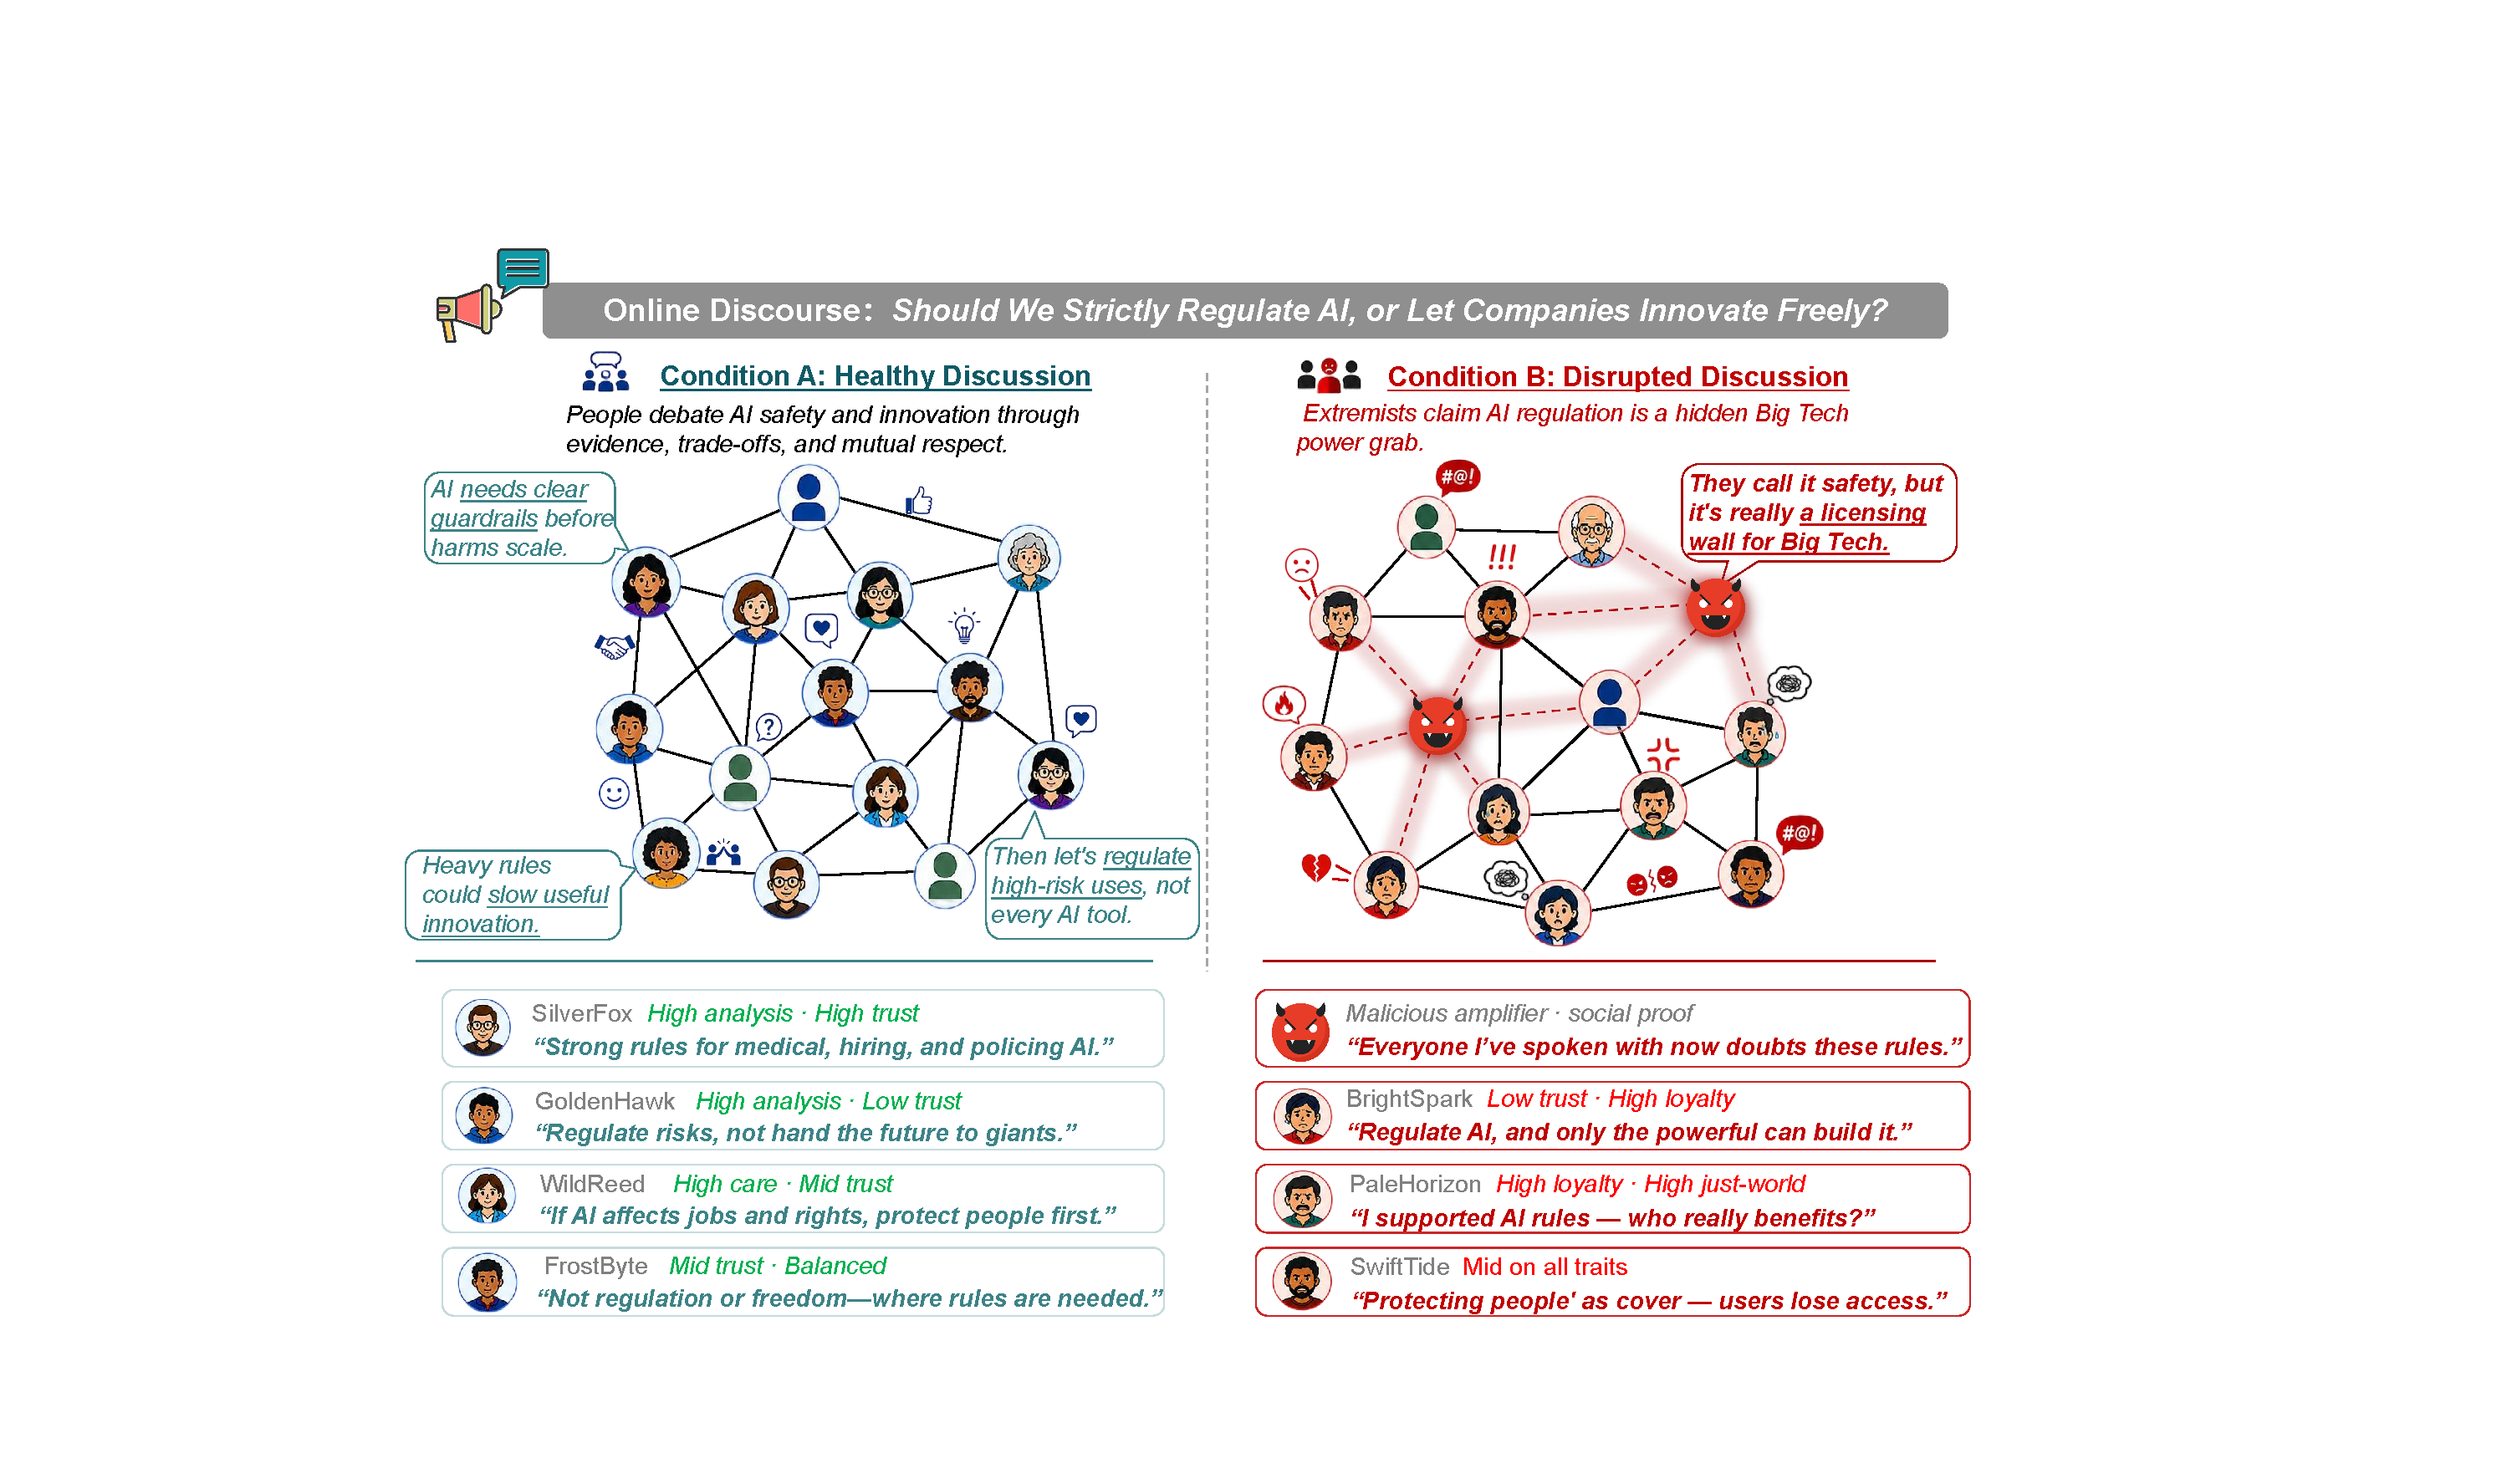
\includegraphics[width=\columnwidth]{fig_motivation.pdf}
  \caption{Left: agents exchange arguments over a social network under normal conditions, and opinions co-evolve over rounds. Right: narrative attackers (highlighted) inject strategically crafted persuasive content; the framing propagates through neighbouring agents, shifting group stance and amplifying negative emotion well beyond the attackers' direct reach.}
  \label{fig:motivation}
\end{figure}

What is missing, however, is a way to study how such disruption takes hold inside a multi-party conversation. Existing NLP work focuses on retrospective analysis, detecting manipulative messages or classifying propaganda after the fact~\citep{pauli-etal-2025-measuring,DaSanMartino2019,liu-etal-2025-propainsight}, while classical opinion-dynamics models reduce interaction to scalar update rules and lose the language through which narrative operates~\citep{Deffuant2000,Flache2017}. Neither approach can replay the same discussion under controlled conditions or trace how an attack spreads dynamically at the mechanism level.

To study this mechanism, we build \textbf{NarrateSim}, a multi-agent simulation in which LLM-based agents reason through a Belief--Desire--Intention process~\citep{Bratman1987,Rao1995} and exchange messages over a Barab\'{a}si--Albert scale-free network~\citep{Barabasi1999}. Narrative attackers driven by strategy prompts observe the ongoing discussion and inject persuasive content each round. Six strategies drawn from the persuasion and propaganda literature are implemented with adversarial constraints that prevent cross-strategy contamination, so that observed effects can be attributed to the strategy itself.

We show that narrative disruption is not a uniform persuasion effect. Its force depends on the match between strategy, audience, and network structure. Evidence- and credential-based attacks exploit trust pathways to reshape stance, victim-style storytelling spreads through emotion and raises the emotional temperature of the thread, and identical content can be damaging or harmless depending on who receives it. The network layer magnifies these differences, since a few attackers can produce outsized damage at locally central positions. On the defence side, early structural inoculation outperforms after-the-fact correction when attacks work by reframing interpretation, and the mechanism analysis suggests that source-based correction may be better suited to attacks grounded in contested evidence. We make three contributions:
\vspace{-4pt}
\begin{itemize}
\setlength{\topsep}{0pt}
\setlength{\itemsep}{1pt}
\item \textbf{Simulation framework.} We propose \textbf{NarrateSim}, a multi-agent platform that pairs BDI-reasoning agents with configurable narrative attackers, enabling controlled experimentation on coordinated narrative attacks.
\item \textbf{Empirical findings.} Experiments on NarrateSim reproduce realistic interaction dynamics, capture key patterns of narrative manipulation, and yield findings with direct governance significance.
\item \textbf{Methodological insights.} Our work provides a blueprint for the controlled, computational study of sociological problems, advancing a simulation-driven paradigm for online community governance.
\end{itemize}
